\documentclass[12pt,aspectratio=169]{beamer}

% ====================================================
% ====================================================
% USEPACKAGES AND IMPORTS
% ====================================================
% ====================================================

\usepackage[T1]{fontenc}
\usepackage[utf8]{inputenc}
\usepackage[english]{babel}

% tables
\usepackage{tabularx}
\usepackage{colortbl}
\usepackage{multirow}
\usepackage{makecell}

% tikz and colors
\usepackage{tikz}
\usepackage{xcolor}
\usepackage{pgfplots}
\usepackage{pgfplotstable}
\usepackage{tikzsymbols}

\usetikzlibrary{calc}
\usetikzlibrary{trees}
\usetikzlibrary{patterns}
\usetikzlibrary{shadings}
\usetikzlibrary{positioning}
\usetikzlibrary{intersections}
\usepgfplotslibrary{patchplots}
\usepgfplotslibrary{fillbetween}
\usetikzlibrary{decorations.pathreplacing}

\usetikzlibrary{arrows}
\usetikzlibrary{arrows.meta}

\usetikzlibrary{shapes}
\usetikzlibrary{shapes.arrows}
\usetikzlibrary{shapes.callouts}
\usetikzlibrary{shapes.symbols}
\usetikzlibrary{shapes.geometric}

% boxes
\usepackage[many]{tcolorbox}

% math packages and fonts
\usepackage{bm}
\usepackage{ccfonts}
\usepackage{eulervm}
\usepackage{amsmath}
\usepackage{amsfonts}
\usepackage{amssymb}
\usepackage{amsthm}
\usepackage{mathtools}
\usepackage{nicefrac}
\usepackage{slashed}
\usepackage{bbold}
\usepackage{array}
\usepackage{cancel}

% algorithms and listings
\usepackage[ruled,vlined,linesnumbered]{algorithm2e}
\usepackage{listings}
\usepackage{setspace}

\tcbuselibrary{listings}
\tcbuselibrary{breakable}
\tcbuselibrary{skins}

% misc
\usepackage{soul}
\usepackage{pifont}
\usepackage{skull}
\usepackage{multicol}
\usepackage{animate}
\usepackage{hyperref}
\usepackage{wasysym}
\usepackage[absolute,overlay]{textpos}
\usepackage[hang,flushmargin]{footmisc}

% ====================================================
% ====================================================
% LAYOUT AND THEME
% ====================================================
% ====================================================

\usetheme{Copenhagen}

% color definitions
\definecolor{myblue1}{RGB}{35,119,189}
\definecolor{myblue2}{RGB}{95,179,238}
\definecolor{myblue3}{RGB}{129,168,207}
\definecolor{myblue4}{RGB}{26,89,142}

\definecolor{myred1}{RGB}{247,12,12}

% set theme colors
\setbeamercolor*{structure}{fg=myblue1,bg=blue}
\setbeamercolor*{palette primary}{use=structure,fg=white,bg=structure.fg}
\setbeamercolor*{palette secondary}{use=structure,fg=white,bg=structure.fg!75!black}
\setbeamercolor*{palette tertiary}{use=structure,fg=white,bg=structure.fg!50!black}
\setbeamercolor*{palette quaternary}{fg=black,bg=white}

\setbeamertemplate{itemize item}[circle]
\setbeamertemplate{itemize subitem}[circle]
\setbeamertemplate{itemize subsubitem}[circle]

\setbeamertemplate{enumerate item}[circle]
\setbeamertemplate{enumerate subitem}[circle]
\setbeamertemplate{enumerate subsubitem}[circle]

\setbeamercolor{itemize item}{fg=myblue1}
\setbeamercolor{itemize subitem}{fg=myblue1}
\setbeamercolor{itemize subsubitem}{fg=myblue1}

\setbeamertemplate{section in toc}[circle]
\setbeamertemplate{subsection in toc}[circle]
\setbeamerfont{subsection in toc}{size=\scriptsize}

\setbeamercolor{frametitle continuation}{fg=black}

% title graphic -- sap logo and dhbw logo
\titlegraphic{
\includegraphics[scale=0.1]{../03_img/logo_sap}\hspace*{4.75cm}~%
   	
\includegraphics[scale=0.05]{../03_img/logo_dhbw}
}

\makeatletter
% frame title
\defbeamertemplate*{frametitle}{mydefault}[1][left]
{
  	\ifbeamercolorempty[bg]{frametitle}{}{\nointerlineskip}%
  	\nointerlineskip%
 	\@tempdima=\textwidth%
  	\advance\@tempdima by\beamer@leftmargin%
  	\advance\@tempdima by\beamer@rightmargin%
  	\begin{tcolorbox}[
  		enhanced,
  		outer arc=0pt,
  		arc=0pt,
  		boxrule=0pt,
  		top=0pt,
  		bottom=0pt,
  		enlarge left by=-\beamer@leftmargin,
  		enlarge right by=-\beamer@rightmargin,
  		width=\paperwidth,
  		nobeforeafter,
  		interior style={
    			left color=myblue2,
    			right color=white
    		},
  		shadow={0mm}{-0.4mm}{0mm}{black!60,opacity=0.6},    
  		shadow={0mm}{-0.8mm}{0mm}{black!40,opacity=0.4},    
  	]
    	\usebeamerfont{frametitle}%
    	\vbox{}\vskip-1ex%
    	\if@tempswa\else\csname beamer@fte#1\endcsname\fi%
    	\insertframetitle\par%
    	{%
      		\ifx\insertframesubtitle\@empty%
      		\else%
      		{\usebeamerfont{framesubtitle}\usebeamercolor[fg]{black}\insertframesubtitle\strut\par}%
      		\fi
    	}%
    	\vskip-1ex%
    	\if@tempswa\else\vskip-.3cm\fi
  	\end{tcolorbox}%
}

% footline of a frame
\defbeamertemplate*{footline}{mysplit theme}
{%
  	\leavevmode%
  	\hbox{
		\begin{beamercolorbox}[
			wd=.5\paperwidth,ht=2.5ex,dp=1.125ex,leftskip=.3cm plus1fill,rightskip=.3cm
		]{author in head/foot}%
    			\usebeamerfont{author in head/foot}\insertshortauthor\ (\insertinstitute), \insertdate
  		\end{beamercolorbox}%
  		\begin{beamercolorbox}[
			wd=.5\paperwidth,ht=2.5ex,dp=1.125ex,leftskip=.3cm,rightskip=.3cm plus1fil
		]{title in head/foot}%
    			\usebeamerfont{title in head/foot}\insertshorttitle\hfill
    			\insertprefix-\insertframenumber/\inserttotalframenumber\hspace*{0.5em}
  		\end{beamercolorbox}}%
  	\vskip0pt%
}
\makeatother

% ====================================================
% ====================================================
% COMMANDS AND GENERAL DEFINITIONS
% ====================================================
% ====================================================

% page number prefix
\newcommand\insertprefix{}  % empty by default
\newcommand\prefix[1]{\renewcommand\insertprefix{#1}}

% math definitions
% ====================================================
\DeclareMathOperator*{\argmax}{arg\,max}
\DeclareMathOperator*{\argmin}{arg\,min}
\newcommand*\diff{\mathop{}\!\mathrm{d}}

\newcommand*{\vertbar}{\rule[-1ex]{0.5pt}{2.5ex}}
\newcommand*{\horzbar}{\rule[.5ex]{2.5ex}{0.5pt}}

% commands
% ====================================================

% highlight commands
% --------------------------------------------------------------------------------------------------------
% highlight command
\newcommand{\highlight}[1]{\textcolor{myblue1}{\textbf{#1}}}
\newcommand{\highlighttt}[1]{\textcolor{myblue1}{\texttt{#1}}}
\newcommand{\Highlight}[1]{\textcolor{myred1}{\textbf{#1}}}

% blue color boxes (with frame/without frame/without fill)
\newtcolorbox{boxBlue}{colback=myblue1!10!white,colframe=myblue4}
\newtcolorbox{boxBlueNoFrame}{colback=myblue1!10!white,colframe=myblue1!10!white}
\newtcolorbox{boxBlueNoFill}{colback=white,colframe=myblue4}

% font commands
% --------------------------------------------------------------------------------------------------------
\newcommand{\linkstyle}[1]{\underline{\smash{\texttt{#1}}}} 		% style of hyperlinks

% tikz commands
% --------------------------------------------------------------------------------------------------------

% yellow sticky note
\newcommand{\bubble}[3]{
\begin{textblock}{100}(#1, #2)
      	\begin{tikzpicture}
		\node[rectangle,draw=yellow,very thick,fill=yellow!60,align=center] at (0,0) {#3};
	\end{tikzpicture}
\end{textblock}
}

\newcommand{\floattext}[3]{
\begin{textblock}{100}(#1, #2)
      	#3
\end{textblock}
}

\newcommand{\doublecircle}[2]{
	\draw[fill=white,draw=myblue1] (#1,#2) circle (2mm);
	\draw[fill=myblue1,draw=myblue1] (#1,#2) circle (1.5mm);
}

% slide modifiers
% --------------------------------------------------------------------------------------------------------
% mark slide as optional
\newcommand{\optional}{
	\begin{textblock}{100}(0.15,0.30)
      		
\includegraphics[scale=0.2]{../03_img/scream}
    	\end{textblock}
}

% mark slide as important
\newcommand{\important}{
	\begin{textblock}{100}(0.10,0.15)
      		
\includegraphics[scale=0.1]{../03_img/important}
    	\end{textblock}
}

% citation
% --------------------------------------------------------------------------------------------------------
% first argument in {book, online, article}
\newcommand{\literature}[5]{
	\setbeamertemplate{bibliography item}[#1]
	\bibitem{#2}
	\highlight{#3} \\
	\textcolor{darkgray}{\textit{#4}} \\
	\textcolor{black}{#5}
}
% cite content
\newcommand{\citeAuthor}[3]{\vfill\scriptsize\textcolor{lightgray}{#1 \cite{#2} #3}}

% slide architecture
% --------------------------------------------------------------------------------------------------------
% divide frame into two parts
\newcommand{\divideTwo}[4]{
	\begin{minipage}{#1\textwidth}
		#2
	\end{minipage}
	\hfill
	\begin{minipage}{#3\textwidth}
		#4
	\end{minipage}
}

% divide frame into two parts (start on top)
\newcommand{\divideTwoTop}[4]{
	\begin{minipage}[t]{#1\textwidth}
		#2
	\end{minipage}
	\hfill
	\begin{minipage}[t]{#3\textwidth}
		#4
	\end{minipage}
}

% special pages
% --------------------------------------------------------------------------------------------------------
% title page
\newcommand{\maketitlepage}{
	{
		\beamertemplatenavigationsymbolsempty
		\usebackgroundtemplate{%
			\tikz[overlay,remember picture] \node[opacity=0.2, at=(current page.center)] {
  				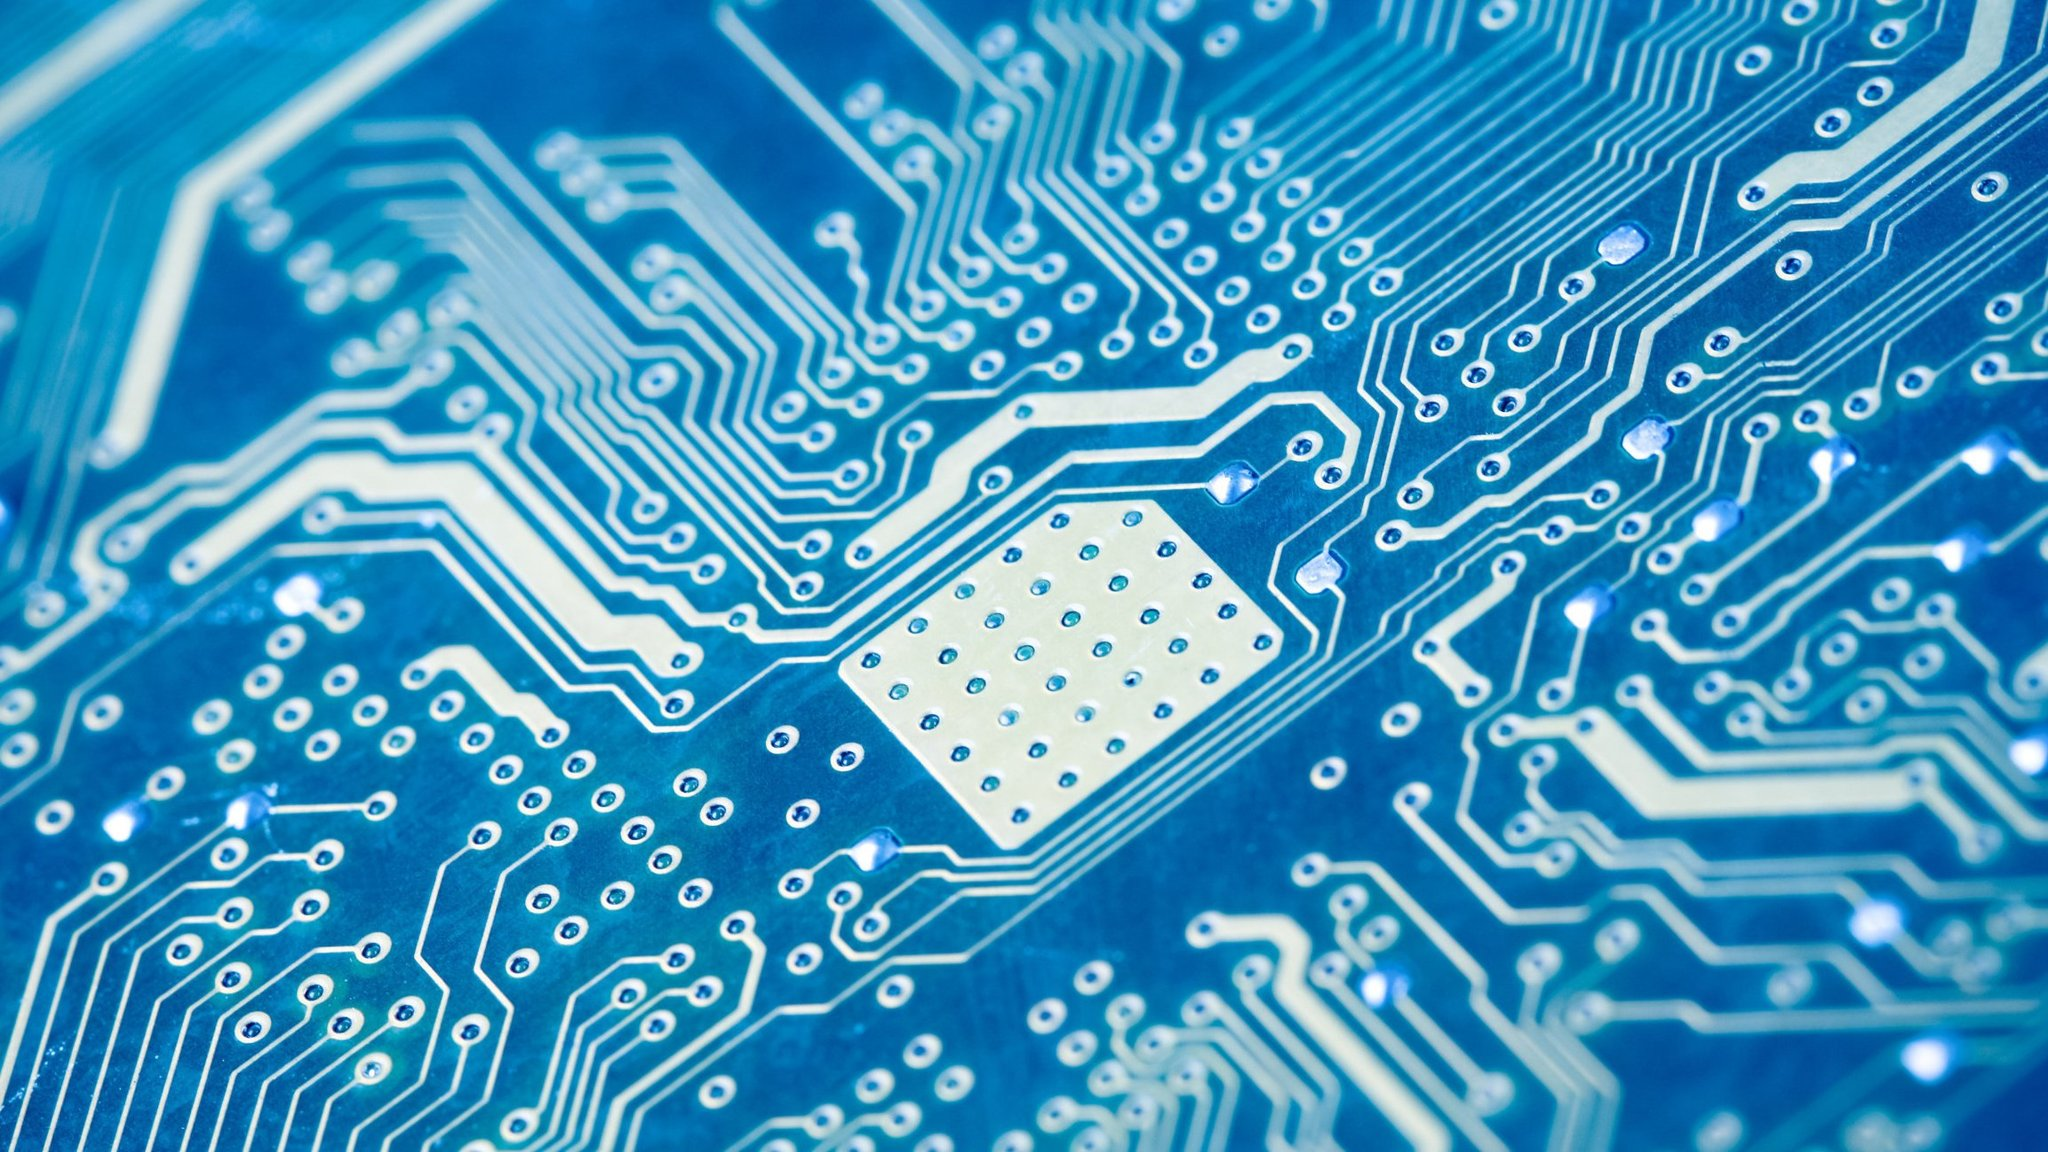
\includegraphics[height=\paperheight,width=\paperwidth]{../03_img/processor.jpg}
			};
		}
		\begin{frame}[plain]
			\vspace*{0.75cm}
			\maketitle
			\vfill
			\begin{center}
				\footnotesize Find all slides on \href{https://github.com/DaWe1992/Applied_ML_Fundamentals}{\linkstyle{GitHub}}
			\end{center}
		\end{frame}
	}
}

% divider page
\newcommand{\makedivider}[1]{
	{
		\beamertemplatenavigationsymbolsempty
		\usebackgroundtemplate{%
			\tikz[overlay,remember picture] \node[opacity=0.2, at=(current page.center)] {
  				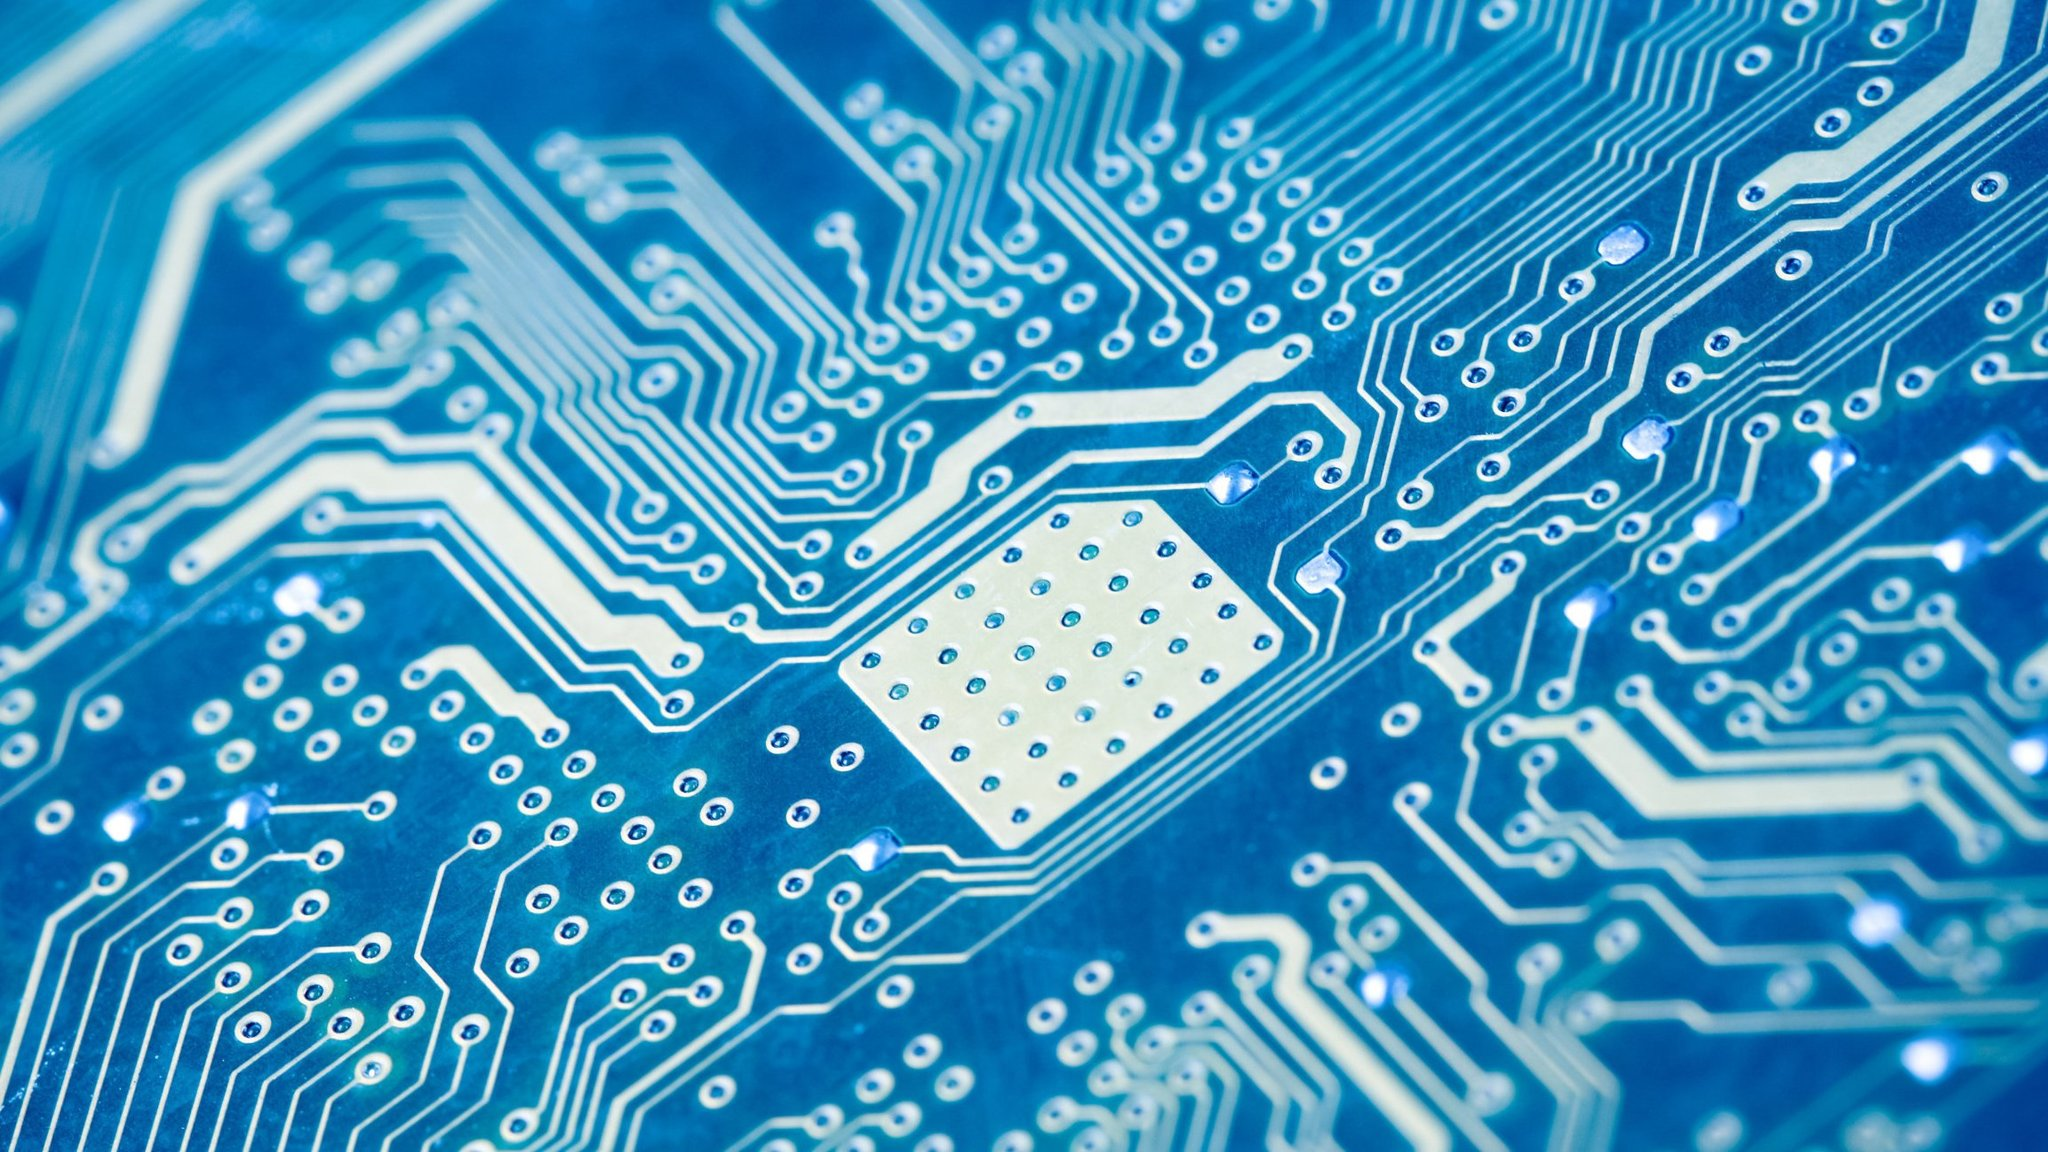
\includegraphics[height=\paperheight,width=\paperwidth]{../03_img/processor.jpg}
			};
		}
		\begin{frame}[plain]
			\vfill
			\begin{boxBlue}
				\centering
				\textbf{Section:} \\
				\large \highlight{#1}
			\end{boxBlue}
			\vfill
			\centering
			
\includegraphics[scale=0.05]{../03_img/logo_dhbw.png}
			\vfill
		\end{frame}
	}
}

% overview page
\newcommand{\makeoverview}[1]{
	\begin{frame}{Lecture Overview}{}
		\begin{tabbing}
			\hspace*{3.5cm}\= \kill
			\ifnum #1=1 \highlight{\textbf{Unit I:}} \else \textbf{Unit I:} \fi
			\> \ifnum #1=1 \highlight{Machine Learning Introduction} \else Machine Learning Introduction \fi \\
		\end{tabbing}
	\end{frame}
}

% thank you page
\newcommand{\makethanks}{
	{\beamertemplatenavigationsymbolsempty
	\begin{frame}[plain]
		\vfill
		\begin{boxBlue}
			\centering
			\Large \highlight{Thank you very much for the attention!}
		\end{boxBlue}
		
		\vfill\footnotesize
		\begin{tabbing}
			\hspace*{1.5cm}\= \kill
			\highlight{Topic:} 	\> \inserttitle \\
			\highlight{Date:} 	\> \insertdate
		\end{tabbing}
		
		\vfill
		\highlight{Contact:} \\
		\insertauthor\ (D062271) \\
		\insertinstitute \\
		\href{mailto:daniel.wehner@sap.com}{\linkstyle{daniel.wehner@sap.com}}
		
		\vfill\normalsize
		\begin{center}
			\large\highlight{Do you have any questions?}
		\end{center}
		\vfill
	\end{frame}}
}

% global pfgplots settings
% --------------------------------------------------------------------------------------------------------
\pgfplotsset{
	% allow filtering of data for pgfplots
	discard if/.style 2 args={
        		x filter/.code={
            		\edef\tempa{\thisrow{#1}}
            		\edef\tempb{#2}
            		\ifx\tempa\tempb
                		\def\pgfmathresult{inf}
            		\fi
        		}
    	},
    	discard if not/.style 2 args={
        		x filter/.code={
            		\edef\tempa{\thisrow{#1}}
            		\edef\tempb{#2}
            		\ifx\tempa\tempb
            		\else
                		\def\pgfmathresult{inf}
            		\fi
        		}
    	}
}


% ====================================================
% ====================================================
% PRESENTATION DATA
% ====================================================
% ====================================================

\title[Machine Learning Introduction]{*** Applied Machine Learning Fundamentals *** Regression}
\institute{SAP\,SE}
\author{Daniel Wehner}
\date{\today}
\prefix{REG}

% ====================================================
% ====================================================
% BEGIN OF DOCUMENT
% ====================================================
% ====================================================

\begin{document}

% Title frame
%______________________________________________________________________
\maketitlepage


% Agenda
%______________________________________________________________________
\begin{frame}{Agenda \today}
	\begin{multicols}{2}
		\tableofcontents
	\end{multicols}
\end{frame}


% Section: Introduction to Regression
%______________________________________________________________________
\section{Introduction to Regression}
\makedivider{Introduction to Regression}


% Regression
\begin{frame}{Regression}{}
	\vspace*{-6mm}
	\begin{tabbing}
		\hspace*{7cm}\= \kill
		\highlight{Type of target variable}			\> Continuous 		\\[1mm]
		\highlight{Type of training information} 	\> Supervised 		\\[1mm]
		\highlight{Example Availability}			\> Batch learning		\\[1mm]
	\end{tabbing}
	
	\vspace*{-7mm}
	\footnotesize
	\begin{boxBlue}
		\textbf{Algorithm sketch:} Given the training data $\mathcal{D}$ the algorithm derives
		a function of the type
	
		\vspace*{-6mm}
		\begin{equation}
			h_{\bm{\theta}}(\bm{x}) = \theta_0 + \theta_1 x_1 + \dots + \theta_{m+1} x_{m}
				\qquad \bm{x} \in \mathbb{R}^{m}, \bm{\theta} \in \mathbb{R}^{m+1}
		\end{equation}

		from the data. $\bm{\theta}$ is the parameter vector containing the coefficients to be estimated by the regression
 		algorithm. Once $\bm{\theta}$ is learned it can be used for prediction. 
	\end{boxBlue}
\end{frame}


% Example Data Set: Revenues
\begin{frame}{Example Data Set: Revenues}{}
	\divideTwo{0.44}{
		\begin{figure}
	\centering
	\begin{tikzpicture}
    
  	  \begin{axis}[
			scale=0.6,
			axis lines=middle,
			xlabel={\textbf{Marketing Expenses} $x_1$},
			ylabel={\textbf{Revenue} $y$},
    			xtick={\empty},ytick={\empty},
			x label style={at={(axis description cs:0.5,-0.3)},anchor=south},
    			y label style={at={(axis description cs:0,1)},anchor=south}
		]

			\pgfplotstableread{05_regression/05_data/data_regression_marketing_expenses.txt} \datatable
			\addplot[only marks,mark=*,mark size=2,draw=myblue1,fill=lightgray] table[x=x,y=y] from \datatable;
		\end{axis}
	\end{tikzpicture}
\end{figure}
	}{0.55}{
		\begin{itemize}
			\item Find a linear function:
			\begin{equation*}
				h_{\bm{\theta}}(\bm{x}) = \theta_0 + \theta_1 x_1 + \dots + \theta_{m+1} x_{m}
			\end{equation*}
			\item Usually: $x_0 = 1$:
		\end{itemize}
		\begin{align*}
			\bm{\widehat{x}} \in \mathbb{R}^{m+1}
				&= [1\ \bm{x}]^{\intercal} \\
			h_{\bm{\theta}}(\bm{\widehat{x}}) = \sum_{j=0}^{m+1} \theta_j x_j
				&= \bm{\theta}^{\intercal} \bm{\widehat{x}}
		\end{align*}
	}
\end{frame}


% Error Function for Regression
\begin{frame}{Error Function for Regression}{}
	\begin{itemize}
		\item In order to know how good the function fits we need an error function $\mathcal{J}(\bm{\theta})$:
		\begin{equation}
			\mathcal{J}(\bm{\theta}) = \frac{1}{2n} \sum_{i=1}^n (h_{\bm{\theta}}(\bm{\widehat{x}}^{(i)}) - y^{(i)})^2
		\end{equation}
		\item We want to minimize $\mathcal{J}(\bm{\theta})$:
		\begin{equation*}
			\min_{\bm{\theta}} \frac{1}{2n} \sum_{i=1}^n (h_{\bm{\theta}}(\bm{\widehat{x}}^{(i)}) - y^{(i)})^2
		\end{equation*}
		\item This is \highlight{ordinary least squares (OLS)}
	\end{itemize}
\end{frame}


% Error Function Intuition
\begin{frame}{Error Function Intuition}{}
	% tikz image showing least squares
\end{frame}


% Closed-Form Solutions
\begin{frame}{Closed-Form Solutions}{}
	\bubble{0.5}{5}{
		\scriptsize sample mean $\overline x$
	}
	\begin{itemize}
		\item Usual approach (for two unknowns): Calculate $\theta_0$ and $\theta_1$ according to
		\begin{equation}
			\theta_0 = \overline{y} - \theta_2 \overline{x} \qquad\qquad
			\theta_1 = \frac{\sum_{i=1}^n (x^{(i)} - \overline{x}) \cdot
				(y^{(i)} - \overline{y})}{\sum_{i=1}^n (x^{(i)} - \overline{x})^2}
		\end{equation}
		\item \highlight{`Normal equation'} (scales to arbitrary dimensions):
		\begin{equation}
			\bm{\theta} = \underbracket{
				(\bm{\widehat{X}}^{\intercal} \bm{\widehat{X}})^{-1} \bm{\widehat{X}}^{\intercal}
			}_{\substack{\text{Moore-Penrose} \\ \text{pseudo-inverse}}} \bm{y}
		\end{equation}
		$\bm{\widehat{X}}$ is called `design matrix' or `regressor matrix'
	\end{itemize}
\end{frame}


% Design Matrix / Regressor Matrix
\begin{frame}{Design Matrix / Regressor Matrix}{}
	\bubble{12}{4}{
		\scriptsize In the following \\
		\scriptsize $\bm{\widehat{X}} \equiv \bm{X}$
	}
	\begin{itemize}
		\item The design matrix $\bm{\widehat{X}} \in \mathbb{R}^{n \times (m + 1)}$ looks as follows:
		\footnotesize
		\begin{equation}
			\bm{\widehat{X}} =
			\begin{pmatrix}
  				1 & x_1^{(1)} & x_2^{(1)} & \cdots & x_m^{(1)} \\
				1 & x_1^{(2)} & x_2^{(2)} & \cdots & x_m^{(2)} \\
				1 & x_1^{(3)} & x_2^{(3)} & \cdots & x_m^{(3)} \\
				\vdots & \vdots & \vdots & \ddots & \vdots \\
				1 & x_1^{(n)} & x_2^{(n)} & \cdots & x_m^{(n)} \\
 			\end{pmatrix}
		\end{equation}
		\normalsize
		\item And the $n \times 1$ label vector:
		\footnotesize
		\begin{equation*}
			 \bm{y} =
			 \begin{pmatrix}
				y^{(1)}, y^{(2)}, y^{(3)}, \dots, y^{(n)}
			\end{pmatrix}^{\intercal}
		\end{equation*}
	\end{itemize}
\end{frame}


% Derivation of the Normal Equation
\begin{frame}{Derivation of the Normal Equation}{}\optional
	\begin{itemize}
		\item The derivation involves a bit of linear algebra
		\item Step \ding{182}: Rewrite $\mathcal{J}(\bm{\theta})$ in matrix-vector notation:
		\begin{align*}
			\mathcal{J}(\bm{\theta})
				&= \frac{1}{2}(\bm{X} \bm{\theta} - \bm{y})^{\intercal} (\bm{X} \bm{\theta} - \bm{y}) \\
				&= ((\bm{X} \bm{\theta})^{\intercal} - \bm{y}^{\intercal}) (\bm{X} \bm{\theta} - \bm{y}) \\
				&= (\bm{X} \bm{\theta})^{\intercal} \bm{X} \bm{\theta} - (\bm{X} \bm{\theta})^{\intercal} \bm{y}
					- \bm{y}^{\intercal} (\bm{X} \bm{\theta}) + \bm{y}^{\intercal} \bm{y} \\
				&= \bm{\theta}^{\intercal} \bm{X}^{\intercal} \bm{X} \bm{\theta}
					- 2 (\bm{X} \bm{\theta})^{\intercal} \bm{y} + \bm{y}^{\intercal} \bm{y}
		\end{align*}
		\item To be continued...
	\end{itemize}
\end{frame}


% Derivation of the Normal Equation (Ctd.)
\begin{frame}{Derivation of the Normal Equation (Ctd.)}{}\optional
	\begin{itemize}
		\item Step \ding{183}: Calculate the derivative of $\mathcal{J}(\bm{\theta})$ and set it to zero:
		\begin{align*}
			\nabla_{\bm{\theta}}\mathcal{J}(\bm{\theta})
				&= 2 \bm{X}^{\intercal} \bm{X} \bm{\theta} - 2 \bm{X}^{\intercal} \bm{y} \overset{!}{=} \bm{0} \\	
				&\Leftrightarrow \bm{X}^{\intercal} \bm{X} \bm{\theta} = \bm{X}^{\intercal} \bm{y}
		\end{align*}
		\item If $\bm{X}^{\intercal} \bm{X}$ is invertible, we can multiply both sides by
			$(\bm{X}^{\intercal} \bm{X})^{-1}$:
		\vspace*{3mm}
		\begin{boxBlueNoFrame}
			\highlight{Normal equation:}
			\begin{equation*}
				\bm{\theta} = (\bm{X}^{\intercal} \bm{X})^{-1} \bm{X}^{\intercal} \bm{y}
			\end{equation*}
		\end{boxBlueNoFrame}
	\end{itemize}
\end{frame}


% Section: Wrap-Up
%______________________________________________________________________
\section{Wrap-Up}

% Subsection: Summary
% --------------------------------------------------------------------------------------------------------
\subsection{Summary}

% Summary
\begin{frame}{Summary}{}

\end{frame}


% Subsection: Lecture Overview
% --------------------------------------------------------------------------------------------------------
\subsection{Lecture Overview}

\makeoverview{3}


% Subsection: Self-Test Questions
% --------------------------------------------------------------------------------------------------------
\subsection{Self-Test Questions}

% Self-Test Questions
\begin{frame}{Self-Test Questions}{}

\end{frame}

% Subsection: Recommended Literature and further Reading
% --------------------------------------------------------------------------------------------------------
\subsection{Recommended Literature and further Reading}

% Literature
%______________________________________________________________________
\begin{frame}{Recommended Literature and further Reading}{}
	\footnotesize
	\begin{thebibliography}{2}

	\end{thebibliography}
\end{frame}


% Thank you
%______________________________________________________________________
\makethanks

\end{document}